\icode{E-MM-SI-L2-261011-001}
静止在光滑水平面上质量为\(m =\) \qty{4}{kg}的物块在水平拉力 $F$ 作用下开始运动，$F$ 随时间变化如图所示。则下列说法正确的是\paren[]

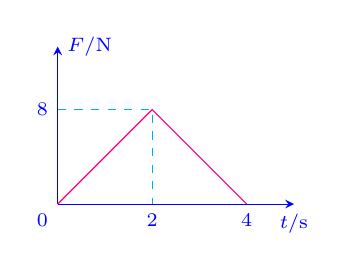
\begin{tikzpicture}[>=stealth,font=\scriptsize]
	\draw[->,blue] (0,0)node[below left]{0}--(3,0)node[below]{\(t\)/\qty{}{s}};
    \draw[->,blue] (0,0)--(0,2)node[right]{\(F\)/\qty{}{N}};
    \draw[dashed,cyan] (0,1.2)node[left,blue]{8}--(1.2,1.2)--(1.2,0)node[below,blue]{2};
	\draw[magenta] (0,0)--(1.2,1.2)--(2.4,0);
	\node at(2.4,0)[below,blue]{4};
\end{tikzpicture}
\begin{choices}
	\item 物块在 $0\sim2$\qty{}{s} 内做匀加速运动，$2\sim4$\qty{}{s} 内做匀减速运动
	\item 物块一直做加速运动，力 $F$ 的功率一直增大
	\item 力 $F$ 在 $0\sim2$\qty{}{s} 内做的功与 $2\sim4$\qty{}{s} 内做的功相等
	\item $0\sim4$\qty{}{s} 内力 $F$ 做功为\qty{32}{J}
\end{choices}
\begin{answer}
    D\qquad 提示：\(F - t\)图像围成的面积是冲量
\end{answer}